\chapter{Pianificazione del progetto} 
\label{cha:pianificazione_del_progetto}	

\section{Introduzione}
\label{sec:introduzione}
In questo documento verrà descritto il processo di sviluppo utilizzato e verrà effettuata la pianificazione delle iterazioni e delle attività da svolgere.
Sarà inoltre fornita una pianificazione temporale del lavoro e sarà possibile verificare lo stato attuale dei lavori consultando questo documento. Infatti manterremo aggiornato questo documento tenendo traccia dell'avanzamento dello sviluppo del sistema.

\section{Processo di sviluppo}
\label{sec:processo_di_sviluppo}
Il progetto sarà realizzato secondo la metodologia di sviluppo \gls{rup}.
Tale motodologia prevede quattro fasi sequenziali che possono essere iterate:
\begin{enumerate}
	\item \fase{Inizio}: fase in cui vengono raccolti i requisiti principali.

	\item \fase{Elaborazione}: fase in cui vengono corretti i requisiti, viene effettuata una analisi ordinata, la progettazione e le prime implementazioni.

	\item \fase{Costruzione}: fase in cui viene completata la progettazione (con i dettagli), viene implementato il sistema e vengono effettuati verifiche e test di aggregazione.

	\item \fase{Transizione}: fase in cui vengono effettuati test finali di pre--produzione, messa in opera, manutenzione, archiviazione documentale e attivazione procedure di gestione.
\end{enumerate}

\noindent
In ognuna di queste fasi possono essere svolte le seguenti attività:
\begin{itemize}
	\item \workflow{Raccolta dei requisiti}
	\item \workflow{Analisi}
	\item \workflow{Progettazione}
	\item \workflow{Implementazione}
	\item \workflow{Test}
\end{itemize}

\noindent
A seconda della fase in cui ci si trova verranno svolte più o meno attività. 
Un tipico esempio di distribuzione delle attività nelle varie fasi è il seguente:
\begin{center}
   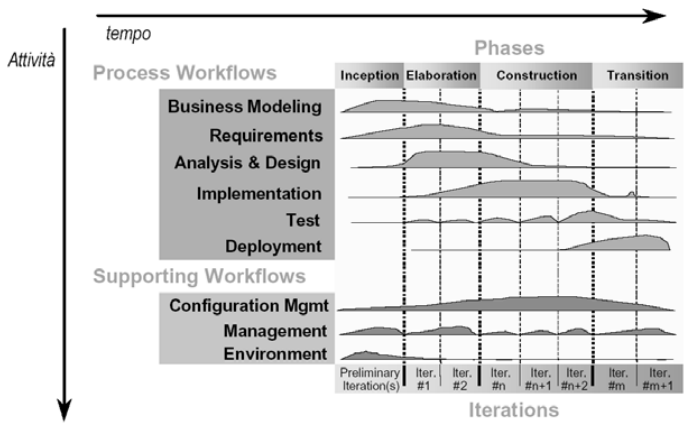
\includegraphics[width= \textwidth]{assets/fasiworkflow}
\end{center}

\section{Pianificazione iterazioni}
\label{sec:pianificazione_iterazioni}
Saranno di seguito elencate le iterazioni svolte durante il progetto, durante lo sviluppo compariranno le iterazioni già effettuate e la pianificazione dell'iterazione successiva.

\begin{center}
	\begin{tabularx}{\tabwidthiter}{ l  X } 
		\toprule
		\multicolumn{2}{c}{\tabtitleiter{Iterazione 01}}  \\
		\cmidrule(l{\cmidrulekern}r{\cmidrulekern}){1-2}
		\tabheaditer{Fase} & Inception \\ 
		\addlinespace[1em] 
		\tabheaditer{Milestone} & 
		    \begin{enumWork}
			        \item Stesura del documento di richiesta
			        \item Stesura del documento di visione
			        \item Stesura dello studio di fattibilità
			        \item Stesura del contratto
			        \item Inizio stesura del glossario
			        \item Inizio stesura del documento di pianificazione del progetto
		    \end{enumWork} \\
		\addlinespace[1em]
		\tabheaditer{Stato} &  In corso \\
		\bottomrule
	\end{tabularx}
\end{center}